\documentclass[11pt]{extarticle}
% Packages
\usepackage{algorithm}  
\usepackage{algorithmicx}  
\usepackage{algpseudocode}
\usepackage{amsmath}
\usepackage{amsthm}
\usepackage{amssymb}
\usepackage{amsfonts}
\usepackage{bm}
\usepackage{caption}
\usepackage{cite}
\usepackage{color}
\usepackage{enumerate}
\usepackage{framed}
\usepackage{graphicx}
\usepackage[hidelinks]{hyperref}
\hypersetup{
    colorlinks=true,
    linkcolor=blue,
    filecolor=magenta,
    urlcolor=cyan,
}
\urlstyle{same}
\usepackage{lipsum}
\usepackage{listings}
\usepackage{multirow}
\usepackage{subcaption}
% \usepackage{subfigure}
\usepackage{tikz}
\usepackage{titlesec}
\usepackage{xcolor}
\usepackage[english]{babel}
\usepackage[utf8]{inputenc}
\usepackage[normalem]{ulem}
\usepackage[top=1 in,bottom=1 in, left=1 in, right=1 in]{geometry}

\usepackage{pgfplots}
\pgfplotsset{compat=newest}
\usepgfplotslibrary{groupplots}
\usepgfplotslibrary{dateplot}

% Settings
\graphicspath{{./Figure/}}
\definecolor{mygreen}{rgb}{0,0.6,0}
\definecolor{mygray}{rgb}{0.5,0.5,0.5}
\definecolor{mymauve}{rgb}{0.58,0,0.82}
\definecolor{lightgray}{gray}{0.95}

\lstset{
    % backgroundcolor = \color{lightgray}, 
    basicstyle = \footnotesize,       
    breakatwhitespace = false,        
    breaklines = true,                 
    captionpos = b,                    
    commentstyle = \color{mygreen}\bfseries,
    emptylines = 1,
    escapeinside = @@,
    extendedchars = false,
    frame = single, 
    framerule = 0.5pt,
    keepspaces = true,
    keywordstyle = \color{mymauve}\bfseries,
    language = python,
    linewidth = \linewidth,
    numbers = left, 
    numbersep = 5pt,
    numberstyle = \tiny\color{mygray},
	otherkeywords = {string},    
    rulecolor = \color{black},         
    showspaces = false,  
    showstringspaces = false,
    showtabs = false,
    stepnumber = 5,         
    stringstyle = \color{mymauve},
    tabsize = 2,
    title = \lstname,
    %xleftmargin = 3em,
}

% A bunch of definitions that make my life easier
\newcommand{\D}{\mathcal{D}}
\newcommand{\N}{\mathcal{N}}
\newcommand{\A}{\mathbf{A}}
\newcommand{\I}{\mathbf{I}}
\newcommand{\T}{\mathbf{T}}
\renewcommand{\t}{\mathbf{t}}
\newcommand{\W}{\mathbf{W}}
\newcommand{\w}{\mathbf{w}}
\newcommand{\X}{\mathbf{X}}
\newcommand{\x}{\mathbf{x}}
\newcommand{\Y}{\mathbf{Y}}
\newcommand{\y}{\mathbf{y}}
\newcommand{\0}{\mathbf{0}}

\renewcommand{\(}{\left(}
\renewcommand{\)}{\right)}

\DeclareMathOperator{\NormalGamma}{NormalGamma}
\DeclareMathOperator{\Gam}{Gam}
\DeclareMathOperator{\Tr}{Tr}

\renewcommand{\vec}{\mathrm{vec}}
\renewcommand{\emptyset}{\varnothing}
% \newcommand{\attn}[1]{\textbf{#1}}
\theoremstyle{definition}
\newtheorem{corollary}{Corollary}
\newtheorem{definition}{Definition}
\newtheorem{example}{Example}
\newtheorem{exercise}{Exercise}
\newtheorem{note}{Note}
\newtheorem{theorem}{Theorem}
\setlength{\columnseprule}{1 pt}
\renewcommand{\algorithmicrequire}{\textbf{Input:}}
\renewcommand{\algorithmicensure}{\textbf{Output:}}  
\newcommand{\image}[3]{
	\begin{figure}[!ht]
		\centering
	    \includegraphics[width=#1\textwidth]{#2}
		\caption{#3}
		\label{fig:#2}
	\end{figure}
}


\title{
    DD2434 Machine Learning, Advanced Course \\
    {\Large Assignment 1}
}
\author{
    Jiang, Sifan \\
	sifanj@kth.se \\
}


\begin{document}
\maketitle
\tableofcontents
\lstlistoflistings

\newpage
\section{Knowing the Rules}
\noindent\fcolorbox{black}{lightgray}{\begin{minipage}{\textwidth}
    \textbf{Question 2.1.1:} \textit{It is mandatory to read the above text. Have you read it?}
\end{minipage}} \\
\par Yes. \\

\noindent\fcolorbox{black}{lightgray}{\begin{minipage}{\textwidth}
    \textbf{Question 2.1.2:} \textit{List all your collaborations concerning the problem formulations in this assignment.}
\end{minipage}} \\
\par Hongsheng Chang. \\

\noindent\fcolorbox{black}{lightgray}{\begin{minipage}{\textwidth}
    \textbf{Question 2.1.3:} \textit{Have you discussed solutions with anybody?}
\end{minipage}} \\


\section{Dependencies in a Directed Graphical Model}
\image{0.5}{Q2_2}{Mixture of components modeling location and strengths of earthquakes associated with a super-epicentra. In the figure, $\mu_{k} = (\mu_{k,1}, \mu_{k,2})$ and $\tau_{k} = (\tau_{k,1}, \tau_{k,2})$.}
%%%%% Question 2.2.4
\noindent\fcolorbox{black}{lightgray}{\begin{minipage}{\textwidth}
    \textbf{Question 2.2.4:} \textit{In the graphical model of Figure \ref{fig:Q2_2}, is $\mu_{k} \perp \tau_{k}$ (not conditioned by anything)?}
\end{minipage}} \\
\par Yes, $\mu_{k} \perp \tau_{k}$ is true.
\begin{align*}
    p(\mu_{k}, \tau_{k}) =& p(\mu_{k})p(\tau_{k})p\left(X^{1}, \cdots, X^{N} \mid \mu_{k}, \tau_{k}\right).
\end{align*}
\par Since none of the variables are observed, after ``marginalizing both sides of'' the above equation over $X^{1}, \cdots, X^{N}$ we obtain \cite{Bishop}:
\begin{align*}
    p(\mu_{k}, \tau_{k}) =& p(\mu_{k})p(\tau_{k}).
\end{align*}
\par So, $\mu_{k} \perp \tau_{k}$. \\

%%%%% Question 2.2.5
\noindent\fcolorbox{black}{lightgray}{\begin{minipage}{\textwidth}
    \textbf{Question 2.2.5:} \textit{In the graphical model of Figure \ref{fig:Q2_2}, is $\mu_{k} \perp \tau_{k} \mid X^{1}, \cdots, X^{N}$?}
\end{minipage}} \\
\par No, $\mu_{k} \perp \tau_{k} \mid X^{1}, \cdots, X^{N}$ is false.
\begin{align*}
    p(\mu_{k}, \tau_{k} \mid X^{1}, \cdots, X^{N}) =& \frac{p\left(\mu_{k}, \tau_{k}, X^{1}, \cdots, X^{N} \right)}{p\left(X^{1}, \cdots , X^{N} \right)} \\
    =& \frac{p(\mu_{k})p(\tau_{k})p\left(X^{1},\cdots,X^{N} \mid \mu_{k}, \tau_{k}\right)}{p\left(X^{1}, \cdots, X^{N}\right)},
\end{align*}
which isn't factorized into the product $p(\mu_{k})p(\tau_{k})$, thus $\mu_{k} \perp \tau_{k} \mid X^{1}, \cdots, X^{N}$ is false.

\image{0.5}{Q2_2_6}{The $K$ super epicentra model with priors.}
%%%%% Question 2.2.6
\noindent\fcolorbox{black}{lightgray}{\begin{minipage}{\textwidth}
    \textbf{Question 2.2.6:} \textit{In the graphical model of Figure \ref{fig:Q2_2_6}, is $\mu \perp b^{'}$ (not conditioned by anything)?}
\end{minipage}} \\
\par No, $\mu \perp b^{'}$ is false.
\begin{align*}
    p(\mu, b^{'}, \tau) = p(b^{'}) p(\tau \mid b^{'}) p(\mu \mid \tau).
\end{align*}
\par By marginalizing over $\tau$, we can obtain
\begin{align*}
    p(\mu, b^{'}) = p(b^{'}) \sum_{\tau} p(\tau \mid b^{'}) p(\mu \mid b^{'}) = p(\mu \mid b^{'}) p(b^{'}),
\end{align*}
which isn't factorized into the product $p(\mu)p(b^{'})$, thus $\mu \perp b^{'}$ is false. \\

%%%%% Question 2.2.7
\noindent\fcolorbox{black}{lightgray}{\begin{minipage}{\textwidth}
    \textbf{Question 2.2.7:} \textit{In the graphical model of Figure \ref{fig:Q2_2_6}, is $\mu \perp b^{'} \mid X^{1}, \cdots, X^{N}$?}
\end{minipage}} \\
\par No. \\

%%%%% Question 2.2.8
\noindent\fcolorbox{black}{lightgray}{\begin{minipage}{\textwidth}
    \textbf{Question 2.2.8:} \textit{In the graphical model of Figure \ref{fig:Q2_2_6}, is $X^{n} \perp S^{n}$ (not conditioned by anything)?}
\end{minipage}} \\
\par No. \\

%%%%% Question 2.2.9
\noindent\fcolorbox{black}{lightgray}{\begin{minipage}{\textwidth}
    \textbf{Question 2.2.9:} \textit{In the graphical model of Figure \ref{fig:Q2_2_6}, is $X^{n} \perp S^{n} \mid \mu_{k}, \tau_{k}$?}
\end{minipage}} \\
\par No.


\section{Likelihood of a tree GM only for E level}


\section{Simple VI}
%%%%% Question 2.4.12
\noindent\fcolorbox{black}{lightgray}{\begin{minipage}{\textwidth}
    \textbf{Question 2.4.12:} \textit{Implement the VI algorithm for the variational distribution in Equation (10.24) in Bishop.}
\end{minipage}} \\
\par From \textit{Bishop} \cite{Bishop}, the variational distribution is given by
\begin{align*}
    q(\mu, \tau) =& q_{\mu}(\mu) q_{\tau}(\tau) \\
    q_{\mu}(\mu) =& \N(\mu \mid \mu_{N}, \lambda_{N}^{-1}) \\
    q_{\tau}(\tau) =& \Gam(\tau \mid a_{N}, b_{N}),
\end{align*}
where
\begin{align*}
    \mu_{N} =& \frac{\lambda_{0}\mu_{0} + N\bar{x}}{\lambda_{0} + N} \\
    \lambda_{N} =& (\lambda_{0} + N) \mathbb{E}\left[\tau\right] \\
    a_{N} =& a_{0} + \frac{N}{2} \\
    b_{N} =& b_{0} + \frac{1}{2} \mathbb{E}_{\mu}\left[\sum_{n=1}^{N}(x_{n}-\mu)^{2} + \lambda_{0}(\mu-\mu_{0})^{2}\right] \\
    =& b_{0} - \left(\sum_{n=1}^{N}x_{n} + \lambda_{0}\mu_{0}\right)\mathbb{E}_{\mu}[\mu] + \frac{1}{2}\left(\sum_{n=1}^{N}x_{n}^{2} + \lambda_{0}\mu_{0}^{2} + (\lambda_{0} + N)\mathbb{E}_{\mu}[\mu^{2}]\right).
\end{align*}
\par Where
\begin{align*}
	\mathbb{E}_{\mu}[\mu] =& \mu_{N} \\
	\mathbb{E}_{\mu}[\mu^{2}] =& \frac{1}{\lambda_{N}} + \mu_{N}^{2} \\
	\mathbb{E}_{\tau}[\tau] =& \frac{a_{N}}{b_{N}}.
\end{align*}
\par Due to non-informative condition, we set $\mu_{0} = \lambda_{0} = a_{0} = b_{0} = 0$. Then the VI algorithm would be an iterative algorithm that start with a set of initial values of $\mu_N$, $\lambda_{N}$, $a_{N}$, and $b_{N}$. Then the values of $\mu_N$, $\lambda_{N}$, $a_{N}$, and $b_{N}$ should be updated to obtain a converging result of approximated posterior distribution. The algorithm is shown in the following code:
\lstinputlisting[caption=Simple VI.]{Code/2_4.py}

%%%%% Question 2.4.13
\noindent\fcolorbox{black}{lightgray}{\begin{minipage}{\textwidth}
    \textbf{Question 2.4.13:} \textit{What is the exact posterior?}
\end{minipage}} \\
\par Since gamma distribution is a conjugate prior of the normal distribution, the joint distribution of the Normal-Gamma distribution is
\begin{align*}
    p(\mu, \tau \mid \mu_{0}, \lambda_{0}, a_{0}, b_{0}) =& \frac{b_{0}^{a_{0}} \sqrt{\lambda_{0}}}{\Gamma(a_{0})\sqrt{2\pi}} \tau^{a_{0}-\frac{1}{2}} \exp\left[-b_{0}\tau\right] \exp\left[-\frac{ \lambda \tau(\mu - \mu_{0})^2}{2}\right] \\
    p(\mu, \tau) \propto& \tau^{a_{0}-\frac{1}{2}} \exp\left[-b_{0}\tau\right] \exp\left[-\frac{ \lambda \tau(\mu - \mu_{0})^2}{2}\right]
\end{align*}
\par According to Bayesian theorem, we have
\begin{align*}
	p(\mu, \tau \mid \D) \propto& p(\D \mid \mu, \tau) p(\mu, \tau),
\end{align*}
where $p(\D \mid \mu, \tau)$ is the likelihood of the data points which have such relationship:
\begin{align*}
	p(\D \mid \mu, \tau) =& \prod_{i=1}^{N} p(x_{i} \mid \mu, \tau) \\
	\propto& \prod_{i=1}^{N} \tau^{1/2} \exp\left[-\frac{\tau}{2}(x_{i} - \mu)^{2}\right] \\
	\propto& \tau^{N/2} \exp\left[-\frac{\tau}{2}\sum_{i=1}^{N}(x_{i} - \mu)^{2}\right] \\
	\propto& \tau^{N/2} \exp\left[-\frac{\tau}{2}\sum_{i=1}^{N}(x_{i} - \bar{x} + \bar{x} - \mu)^{2}\right] \\
	\propto& \tau^{N/2} \exp\left[-\frac{\tau}{2}\sum_{i=1}^{N}\((x_{i}-\bar{x})^{2}+(\bar{x}-\mu)^{2}\)\right] \\
	\propto& \tau^{N/2} \exp\left[-\frac{\tau}{2}\(Ns+N(\bar{x}-\mu)^{2}\)\right],
\end{align*}
where $\bar{x} = \frac{1}{N}\sum_{i=1}^{N}x_{i}$ and $s = \frac{1}{N}\sum_{i=1}^{N}(x_{i}-\mu)^{2}$. Thus the posterior can be written into \cite{Doing}
\begin{align*}
	p(\mu, \tau \mid \D) \propto& p(\D \mid \mu, \tau) p(\mu, \tau) \\
	\propto& \tau^{N/2} \exp\left[-\frac{\tau}{2}\(Ns+N(\bar{x}-\mu)^{2}\)\right] \tau^{a_{0}-\frac{1}{2}} \exp\left[-b_{0}\tau\right] \exp\left[-\frac{ \lambda \tau(\mu - \mu_{0})^2}{2}\right] \\
	\propto& \tau^{\frac{N}{2} + a_{0} - \frac{1}{2}} \exp\left[-\tau\left(\frac{1}{2}Ns + b_{0}\right)\right]\exp\left[-\frac{\tau}{2}\left(\lambda_{0}(\mu - \mu_{0})^{2} + N(\bar{x} - \mu)^{2}\right)\right].
\end{align*}
\par The exponent (except the $-\frac{\tau}{2}$) in the last exponential term can be simplified into
\begin{align*}
	\lambda_{0}(\mu - \mu_{0})^{2} + N(\bar{x} - \mu)^{2} =& \lambda_{0} \mu^{2} - 2\lambda_{0}\mu\mu_{0} + \lambda_{0}\mu_{0}^{2} + N\mu^{2} - 2N\bar{x}\mu + N\bar{x}^{2} \\
	=& (\lambda_{0} + N)\mu^{2} - 2(\lambda_{0}\mu_{0} + N\bar{x})\mu + \lambda_{0}\mu_{0}^{2} + N\bar{x}^{2} \\
	=& (\lambda_{0} + N)\left( \mu^{2} - 2\frac{\lambda_{0}\mu_{0} + N\bar{x}}{\lambda_{0} + N}\mu \right) + \lambda_{0}\mu_{0}^{2} + N\bar{x}^{2} \\
	=& (\lambda_{0} + N)\left( \mu - \frac{\lambda_{0}\mu_{0} + N \bar{x}}{\lambda_{0} + N} \right)^{2} + \lambda_{0}\mu_{0}^{2} + N\bar{x}^{2} - \frac{(\lambda_{0}\mu_{0} + N\bar{x})^{2}}{\lambda_{0} + N} \\
	=& (\lambda_{0} + N)\left( \mu - \frac{\lambda_{0}\mu_{0} + N\bar{x}}{\lambda_{0} + N} \right)^{2} + \frac{\lambda_{0}N(\bar{x} - \mu_{0})^{2}}{\lambda_{0} + N}.
\end{align*}
\par Insert the above equation into the posterior distribution, we have
\begin{align*}
	p(\mu, \tau \mid \D) \propto& \tau^{\frac{N}{2} + a_{0} - \frac{1}{2}} \exp\left[-\tau\left(\frac{1}{2}Ns + b_{0}\right)\right] \exp\left[-\frac{\tau}{2}\left( (\lambda_{0} + N)\left( \mu - \frac{\lambda_{0}\mu_{0} + N\bar{x}}{\lambda_{0} + N} \right)^{2} + \frac{\lambda_{0}N(\bar{x} - \mu_{0})^{2}}{\lambda_{0} + N} \right)\right] \\
	\propto& \tau^{\frac{N}{2} + a_{0} - \frac{1}{2}} \exp\left[-\tau\left(\frac{1}{2}Ns + b_{0} + \frac{\lambda_{0}N(\bar{x} - \mu_{0})^{2}}{2(\lambda_{0} + N)}\right)\right] \exp\left[-\frac{\tau}{2} (\lambda_{0} + N)\left( \mu - \frac{\lambda_{0}\mu_{0} + N\bar{x}}{\lambda_{0} + N} \right)^{2} \right],
\end{align*}
which is in the form of a Normal-Gamma distribution, thus the exact posterior is
\begin{align*}
	p(\mu, \tau \mid \D) =& \NormalGamma(\mu', \lambda', a', b') \\
	\mu' =& \frac{\lambda_{0}\mu_{0} + N\bar{x}}{\lambda_{0} + N} \\
	\lambda' =& \lambda_{0} + N \\
	a' =& a_{0} + \frac{N}{2} \\
	b' =& b_{0} + \frac{1}{2}\left(Ns + \frac{\lambda_{0}N(\bar{x} - \mu_{0})^{2}}{\lambda_{0} + N}\right).
\end{align*}

%%%%% Question 2.4.14
\noindent\fcolorbox{black}{lightgray}{\begin{minipage}{\textwidth}
    \textbf{Question 2.4.14:} \textit{Compare the inferred variational distribution with the exact posterior. Run the inference on data points drawn from iid Gaussians. Do this for three interesting cases and visualize the results. Describe the differences.}
\end{minipage}} \\
\begin{enumerate}
	\item In this case, the number of data set is $N = 10$ and the initial values are $b_{N} = 5$ and $\lambda_{N} = 5$. The result is shown in fig~\ref{fig:2_4_1}, where the true posterior distribution is shown by the colorful contour lines, while the approximated distribution given by the VI algorithm is shown in blue contour lines and red contour lines when reached convergence.
	\begin{figure}[!ht]
		\centering
		\begin{subfigure}{.4\textwidth}
			\centering
			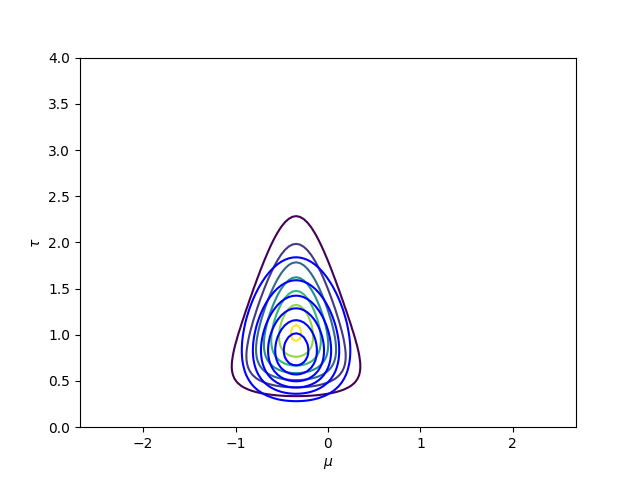
\includegraphics[width=\linewidth]{2_4_1_1}
		\end{subfigure}
		\begin{subfigure}{.4\textwidth}
			\centering
			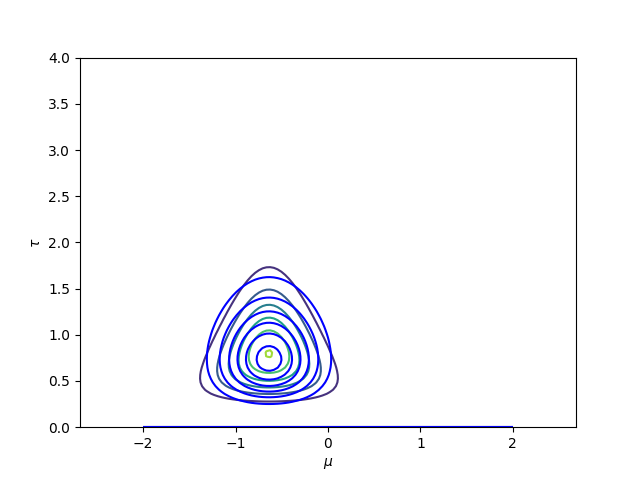
\includegraphics[width=\linewidth]{2_4_1_2}
		\end{subfigure}
		\begin{subfigure}{.4\textwidth}
			\centering
			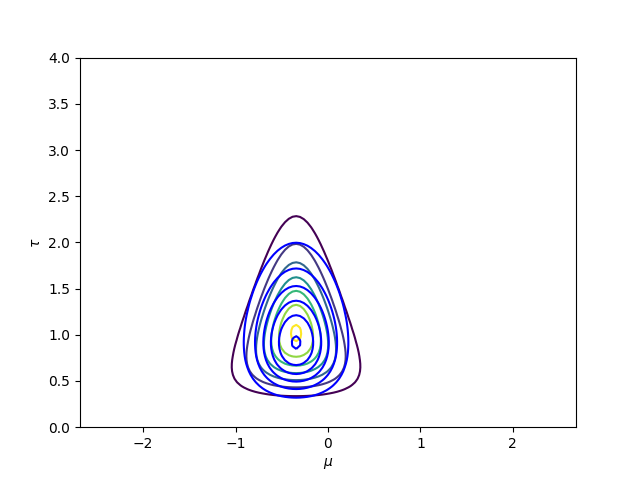
\includegraphics[width=\linewidth]{2_4_1_3}
		\end{subfigure}
		\begin{subfigure}{.4\textwidth}
			\centering
			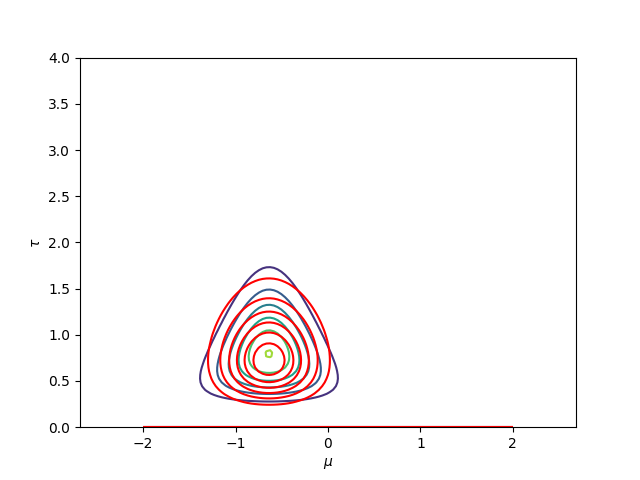
\includegraphics[width=\linewidth]{2_4_1_6}
		\end{subfigure}
		\caption{Simple VI with $\mu_{0} = \lambda_{0} = a_{0} = b_{0} = 0$, $b_{N} = 5$, and $\lambda_{N} = 5$.}
		\label{fig:2_4_1}
	\end{figure}
	\par Although we are using zero for parameters in the prior distributions, so that $\mu_{0} = \lambda_{0} = a_{0} = b_{0} = 0$, which implies that we have no information about the distribution, the convergence is really quick with VI algorithm.
	\par And not only from this case, but also from the following cases, we can see that the mean of the $\mu$ is always correct, which is true since we get value $\mu_{N}$ at the beginning and don't update it during the iterations.

	\item In this case, the number of data set is $N = 10$ and the initial values are $b_{N} = 0.1$ and $\lambda_{N} = 0.1$. The result is illustrated in fig~\ref{fig:2_4_2}.
	\begin{figure}[!ht]
		\centering
		\begin{subfigure}{.4\textwidth}
			\centering
			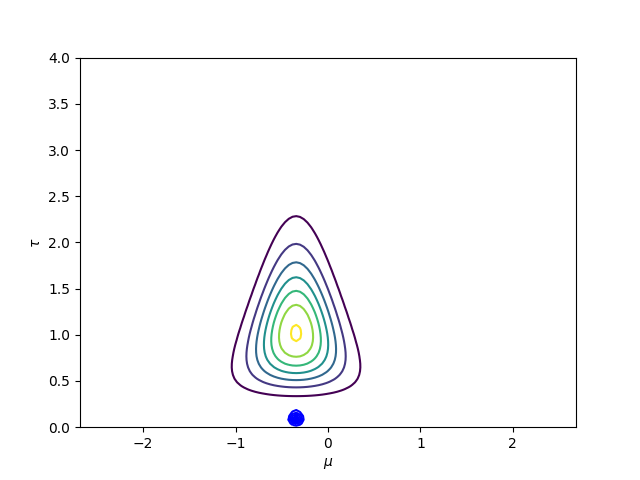
\includegraphics[width=\linewidth]{2_4_2_1}
		\end{subfigure}
		\begin{subfigure}{.4\textwidth}
			\centering
			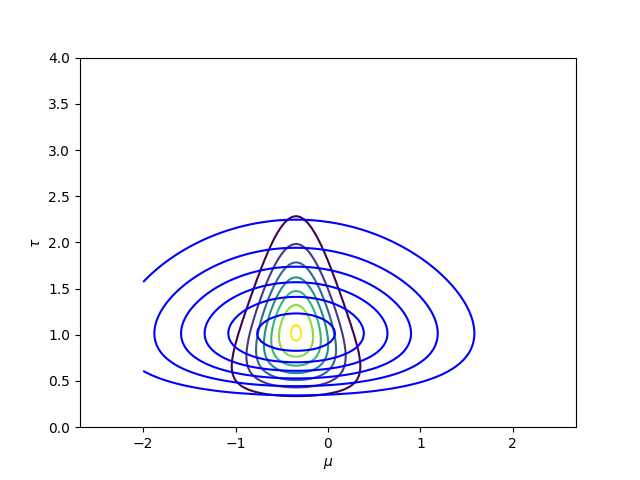
\includegraphics[width=\linewidth]{2_4_2_2}
		\end{subfigure}
		\begin{subfigure}{.4\textwidth}
			\centering
			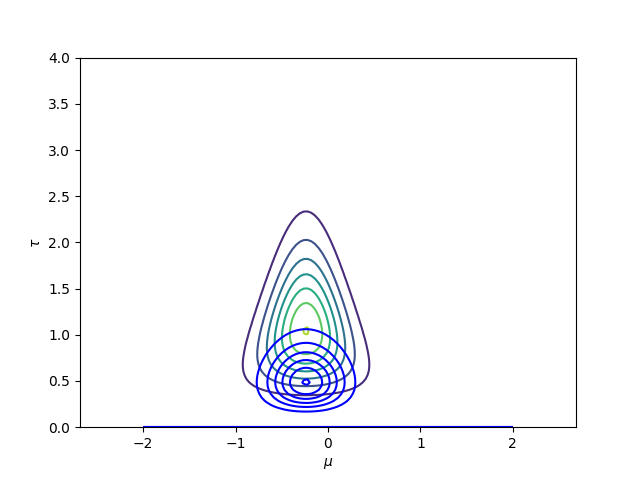
\includegraphics[width=\linewidth]{2_4_2_3}
		\end{subfigure}
		\begin{subfigure}{.4\textwidth}
			\centering
			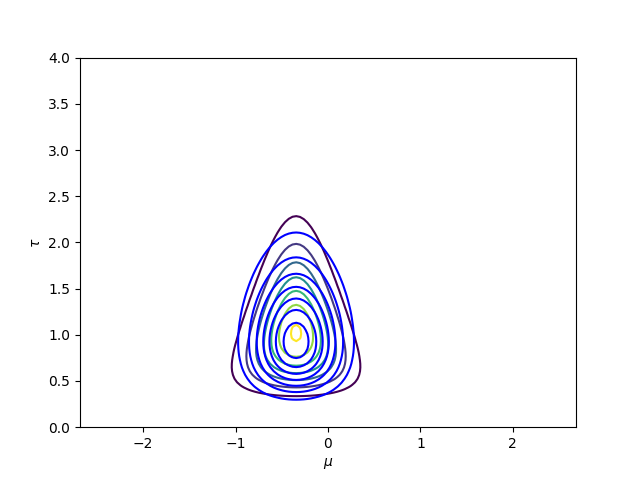
\includegraphics[width=\linewidth]{2_4_2_6}
		\end{subfigure}
		\caption{Simple VI with $\mu_{0} = \lambda_{0} = a_{0} = b_{0} = 0$, $b_{N} = 0.1$, and $\lambda_{N} = 0.1$.}
		\label{fig:2_4_2}
	\end{figure}
	\par By setting the value of the initial values $b_{N}$ and $\lambda_{N}$ to smaller values which are much different to the true values in the true posterior distribution, the converging procedure is slower and requires more iterations to reach the convergence.
	
	\item In this case, the number of data set is $N = 100$ and the initial values are $b_{N} = 5$ and $\lambda_{N} = 5$. The result is illustrated in fig~\ref{fig:2_4_3}.
	\begin{figure}[!ht]
		\centering
		\begin{subfigure}{.4\textwidth}
			\centering
			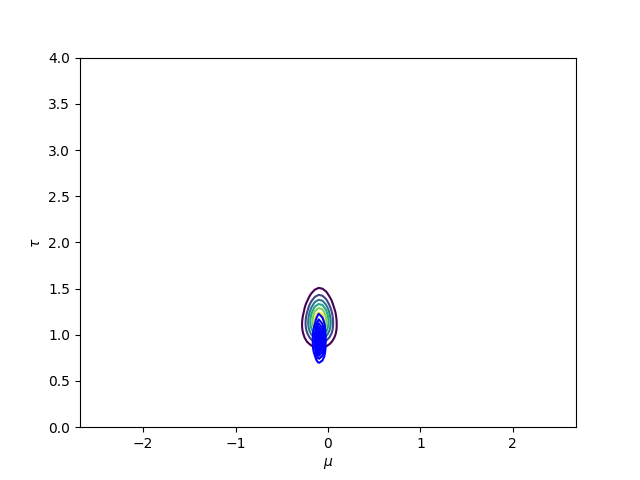
\includegraphics[width=\linewidth]{2_4_3_1}
		\end{subfigure}
		\begin{subfigure}{.4\textwidth}
			\centering
			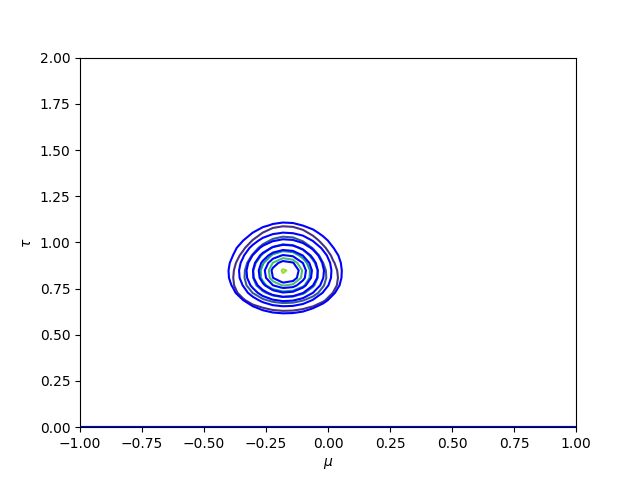
\includegraphics[width=\linewidth]{2_4_3_2}
		\end{subfigure}
		\begin{subfigure}{.4\textwidth}
			\centering
			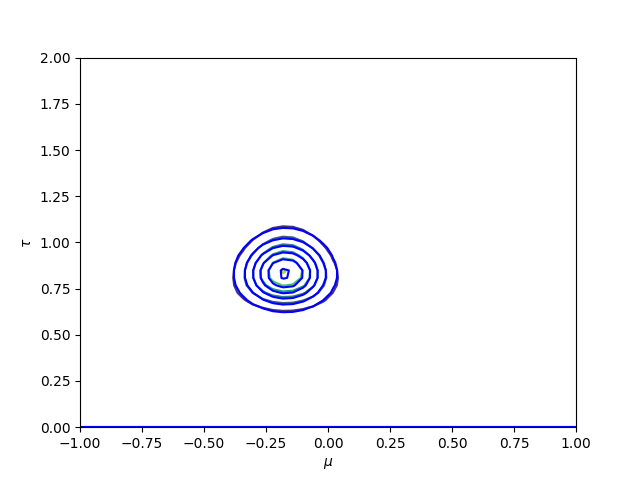
\includegraphics[width=\linewidth]{2_4_3_3}
		\end{subfigure}
		\begin{subfigure}{.4\textwidth}
			\centering
			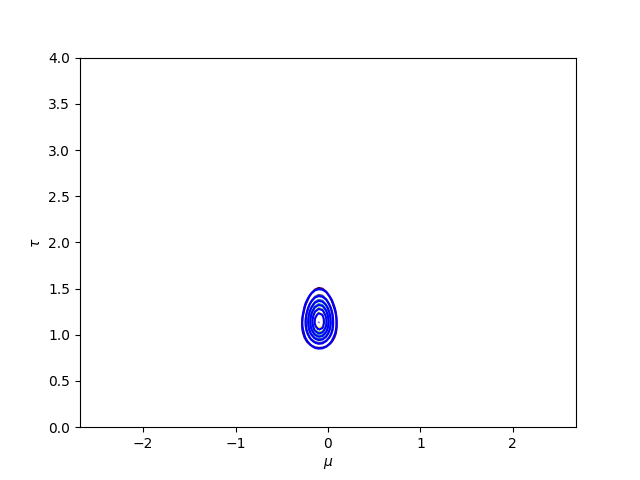
\includegraphics[width=\linewidth]{2_4_3_6}
		\end{subfigure}
		\caption{Simple VI with $\mu_{0} = \lambda_{0} = a_{0} = b_{0} = 0$, $b_{N} = 5$, and $\lambda_{N} = 5$.}
		\label{fig:2_4_3}
	\end{figure}
	\par In this case, we use $100$ data sets generated from a normal distribution. The true posterior distribution for $\mu$ and $\tau$ looks more like a circular shape. And since we have more data sets, we would be confident to the result and the convergence is quick at the same time.
\end{enumerate}


\section{Mixture of trees with observable variables}
%%%%% Question 2.5.15
\noindent\fcolorbox{black}{lightgray}{\begin{minipage}{\textwidth}
    \textbf{Question 2.5.15:} \textit{Implement this EM algorithm.}
\end{minipage}} \\
\par For each $n,k$ the responsibilities is
\begin{align*}
	r_{n,k} =& \frac{\pi_{k}p(x^{n} \mid T_{k}, \Theta_{k})}{p(x^{n})} \\
	=& \frac{\pi_{k}p(x^{n} \mid T_{k}, \Theta_{k})}{\sum_{k=1}^{K} \pi_{k}p(x^{n} \mid T_{k}, \Theta_{k})}.
\end{align*}
\par The algorithm is implemented below, where the function in \textit{Kruskal\_v1.py} is slightly modified so that the result of the maximum spanning tree can be returned:
\lstinputlisting[caption=EM algorithm for mixture of trees with observable variables.]{Code/2_5.py}

%%%%% Question 2.5.16
\noindent\fcolorbox{black}{lightgray}{\begin{minipage}{\textwidth}
    \textbf{Question 2.5.16:} \textit{*}
\end{minipage}} \\

%%%%% Question 2.5.17
\noindent\fcolorbox{black}{lightgray}{\begin{minipage}{\textwidth}
    \textbf{Question 2.5.17:} \textit{*}
\end{minipage}} \\


\section{Super epicentra - EM}
%%%%% Question 2.6.18
\noindent\fcolorbox{black}{lightgray}{\begin{minipage}{\textwidth}
    \textbf{Question 2.6.18:} \textit{Derive an EM algorithm for the model.}
\end{minipage}} \\

%%%%% Question 2.6.19
\noindent\fcolorbox{black}{lightgray}{\begin{minipage}{\textwidth}
    \textbf{Question 2.6.19:} \textit{Implement your EM algorithm.}
\end{minipage}} \\

%%%%% Question 2.6.20
\noindent\fcolorbox{black}{lightgray}{\begin{minipage}{\textwidth}
    \textbf{Question 2.6.20:} \textit{*}
\end{minipage}} \\


\section{Super epicentra - VI}


\section{Sampling from a tree GM}


\section{Failing components VI}

\newpage
\bibliographystyle{ieeetr}
\bibliography{Reference.bib}
\end{document}